\documentclass{simple}

\title[Cum să cucerești lumea]{Cum să cucerești lumea?}
\institute{InfoEducație 2024 (CNU, Focșani)
\author[Răzvan Deaconescu]{Răzvan Deaconescu \\
razvan.deaconescu@upb.ro}
\date{2 august 2024}

\begin{document}

\frame{\titlepage}

\begin{frame}{Care este scopul / sensul vieții?}
  \begin{itemize}
    \pause \item ,,singurul scop al vieții e să-i găsești un sens''
    \pause \item pursuit of happiness
    \pause \item să gustăm din viață pentru viața de apoi
    \pause \item nu există, viața e suferință
    \pause \item ,,Sensul vieții este să-ți găsești darul. Scopul vieții este să-l dăruiești.'' (\textit{Pablo Picasso})
  \end{itemize}
\end{frame}

\begin{frame}{Care este scopul / sensul vieții?}
  \centering
  \textit{But just as a toaster used as a doorstop is still a machine designed to toast bread, you - whatever you choose to do with your life - are still a machine designed to propagate your genes. All of us are. It's what the priests, the sages and philosophers searched for in vain: the ultimate explanation for our existence.}\\
  \vspace{3mm}
  \hfill \textit{Steve Stewart-Williams, The Ape that Understood the Universe: How the Mind and Culture Evolve}
\end{frame}

\begin{frame}{Sclavii ,,evoluției''}
  \begin{itemize}
    \pause \item \textit{natural selection} - supraviețuire
    \pause \item \textit{sexual selection} - perpetuare
    \pause \item \textbf{expansiune}
  \end{itemize}
\end{frame}

\begin{frame}{4X Games}
  \begin{itemize}
    \pause \item explore
    \pause \item expand
    \pause \item exploit
    \pause \item exterminate
  \end{itemize}
\end{frame}

\begin{frame}{Cucerirea lumii}
  \begin{itemize}
    \pause \item vrem să dominăm
    \pause \item vrem să cucerim
    \pause \item vrem să avem impact
    \pause \item vrem să facem istorie
    \pause \item vrem să rămânem în istorie
  \end{itemize}
\end{frame}

\begin{frame}{Cum au cucerit alții lumea?}
  \begin{itemize}
    \pause \item Genghis Khan
    \pause \item Napoleon Bonaparte
    \pause \item Robert Oppenheimer
    \pause \item Elvis Presley
    \pause \item Elon Musk
  \end{itemize}
\end{frame}

\begin{frame}{Ce-a rămas? Ce-a însemnat?}
  \begin{itemize}
    \pause \item ideea celui mai mare imperiu terestru și atât
    \pause \item codul napoleonian, transmiterea idealurilor revoluției franceze / dublu exil și moarte
    \pause \item bomba atomică / relații eșuate, concediat
    \pause \item The King, revoluție muzicală / droguri, relații eșuate, moarte din droguri
    \pause \item companii, avans tehnologic / relații ciudate, ranting cel puțin dubios pe social media, implicare politică
  \end{itemize}
\end{frame}

\begin{frame}{Sunt acești oameni modele? Sunt repere? Se putea mai bine?}
  \begin{itemize}
    \item Genghis Khan
    \item Napoleon Bonaparte
    \item Robert Oppenheimer
    \item Elvis Presley
    \item Elon Musk
  \end{itemize}
\end{frame}

\begin{frame}{}
  \centering
  \pause Lots of energy. \\
  \vspace{3mm}
  \pause But something is not right
\end{frame}

\begin{frame}{}
  \begin{figure}
    \centering
    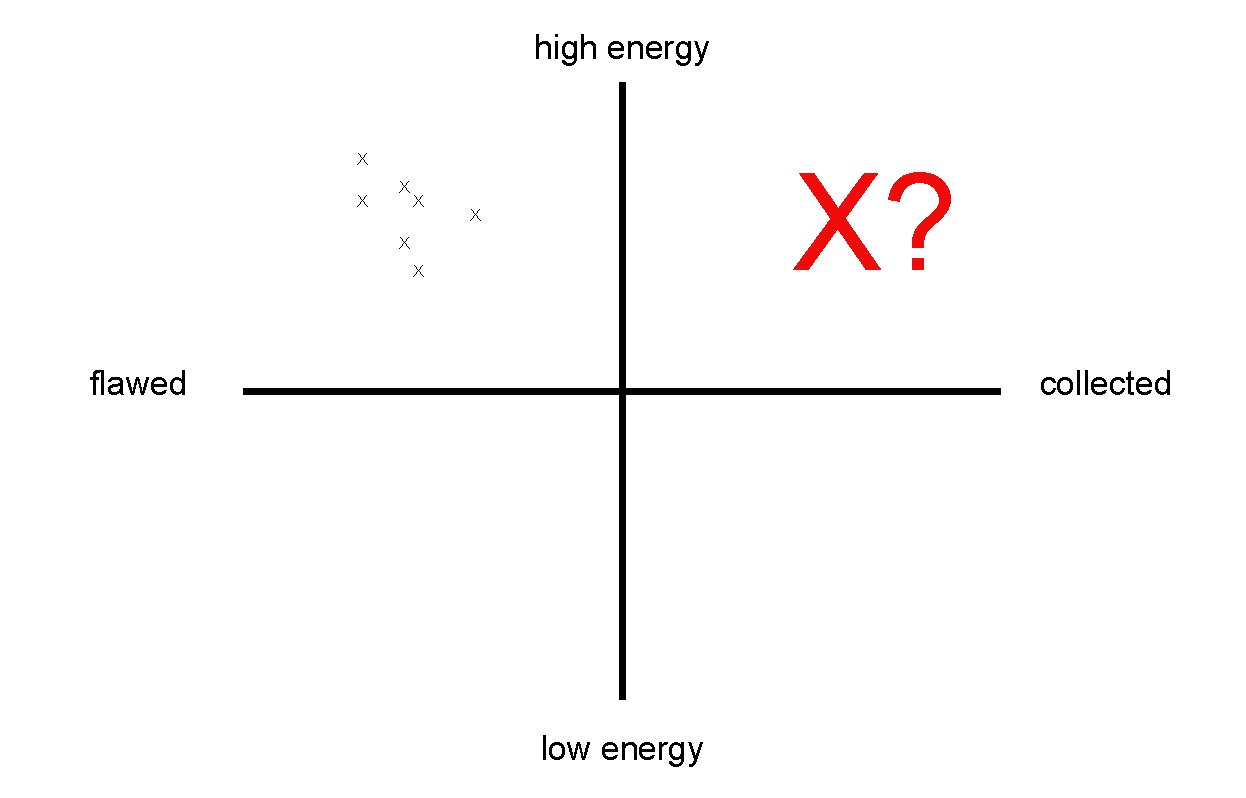
\includegraphics[width=\textwidth]{img/flawed-energy}
  \end{figure}
\end{frame}

\begin{frame}{John D. Rockefeller}
  \centering
  \pause \textit{... was an American business magnate and philanthropist. He was one of the wealthiest Americans of all time[1][2][3][4] and one of the richest people in modern history.}\\
  \vspace{3mm}
  \pause \textit{... was the most successful businessman of all time. He was also a recluse, spending most of his time by himself. He rarely spoke, deliberately making himself inaccessible and staying quiet when you caught his attention.}\\
  \vspace{3mm}
  \pause \textit{ When asked about his silence during meetings, Rockefeller often recited a poem:\\
  A wise old owl lived in an oak,\\
  The more he saw the less he spoke,\\
  The less he spoke, the more he heard,\\
  Why aren't we all like that old bird?}\\
  \hfill \textit{Morgan Housel: \url{https://collabfund.com/blog/lazy-work-good-work/}}
\end{frame}

\begin{frame}{}
  \begin{figure}
    \centering
    
\includegraphics[width=0.7\textwidth]{img/hatred-discipline}
  \end{figure}
\end{frame}

\begin{frame}{}
  \begin{figure}
    \centering
    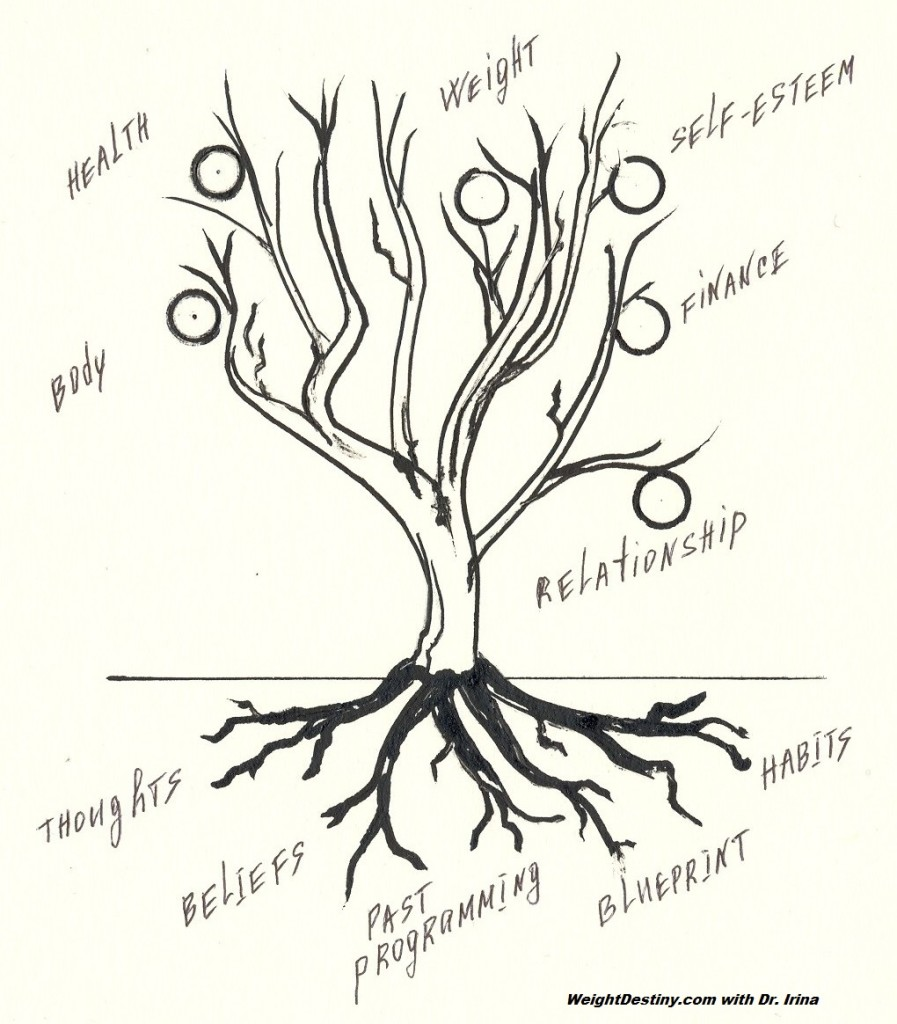
\includegraphics[width=0.7\textwidth]{img/life-tree}
  \end{figure}
\end{frame}

\begin{frame}{}
  \begin{figure}
    \centering
    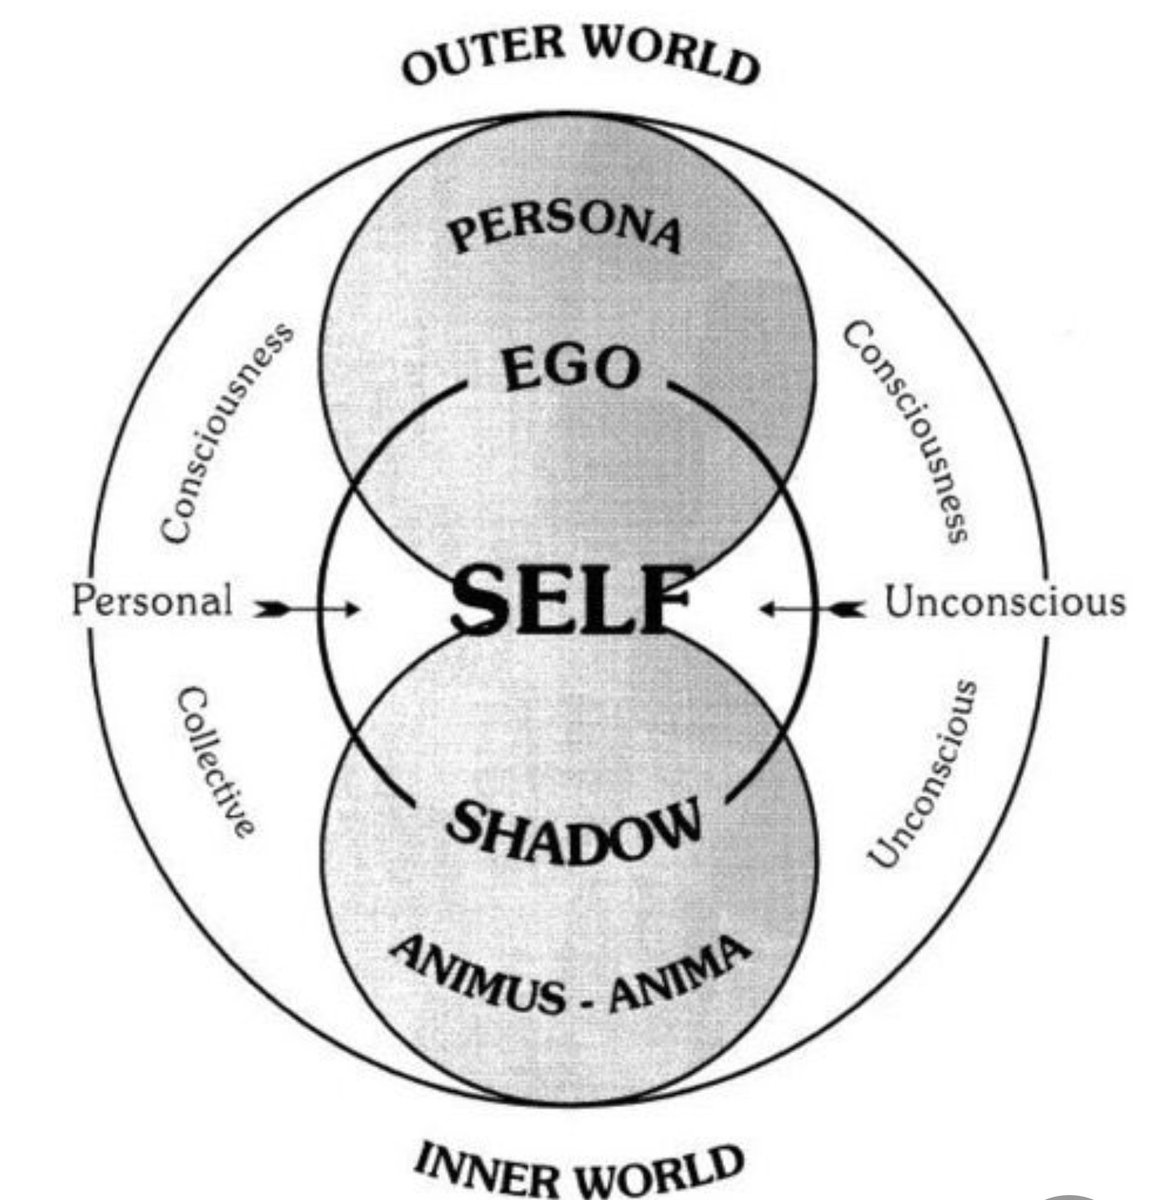
\includegraphics[width=0.7\textwidth]{img/outer-world-inner-world}
  \end{figure}
\end{frame}

\begin{frame}{}
  \centering
  \pause 1. Cucerirea sinelui \\
  \vspace{3mm}
  \pause 2. Cucerirea lumii
\end{frame}

\begin{frame}{}
  \centering
  \pause Ai o discuție cu cineva. \\
  \vspace{3mm}
  \pause Acea persoană îți vorbește despre X. \\
  \vspace{3mm}
  \pause Despre ce vorbește acea persoană?
\end{frame}

\begin{frame}{Situații}
  \begin{itemize}
    \pause \item "Bă, ce prost ești! Cum poți fi așa de prost?"
    \pause \item "N-o să reușești nimic în viață."
    \pause \item "Mi-ai stricat viața."
    \pause \item "Nu-mi place de tine."
    \pause \item \textit{You do not belong here. I have guarded the Trident against false kings since the beginning and for a thousand years. I have seen the greatest champions try and failed, but never have I sensed one as unworthy as you. You dare to come here with your tainted mongrel blood to claim Atlantis's greatest treasure?} (Aquaman, 2018)
  \end{itemize}
\end{frame}

\begin{frame}{Ce fac oamenii cu tine?}
  \begin{itemize}
    \pause \item își proiectează propriile lipsuri, defecte, neajunsuri, traume, păcate
    \pause \item te testează
    \pause \item te folosesc ca ,,sac de box'' al furiei, frustrărilor și anxietăților lor
    \pause \item nu sunt compatibili cu tine, nu vibrează cu tine
    \pause \item pe scurt ... nu e despre tine
  \end{itemize}
\end{frame}

\begin{frame}{\textbf{Ce} înseamnă cucerirea \sout{lumii} sinelui?}
  \begin{itemize}
    \pause \item gestiunea ego-ului
    \pause \item controlul emoțiilor
    \pause \item nuanțarea principiilor, valorilor credințelor; adaptarea la context
    \pause \item ,,detașarea'' de ceilalți, \textit{self-owned}
  \end{itemize}
\end{frame}

\begin{frame}{\textbf{Cum} cucerești \sout{lumea} sinele?}
  \begin{itemize}
    \pause \item deschidere la feedback
    \pause \item meditații, day dreaming, time alone
    \pause \item folosirea simțurilor: ascultă, privește, observă, constată, simte
    \pause \item nu te compara pentru a fi mai bun decât celălalt, compară-te pentru a fi mai bun decât ești acum
    \pause \item ai răbdare, ai multă răbdare, ai foarte foarte multă răbdare
    \pause \item dă mai departe
  \end{itemize}
\end{frame}

\begin{frame}{De avut în vedere}
  \begin{itemize}
    \pause \item it takes time
    \pause \item it never ends
    \pause \item enjoy the process
  \end{itemize}
\end{frame}

\begin{frame}{}
  \begin{itemize}
    \pause \item Nu cred în perfecțiune. Cred în perfectibilitate.
    \pause \item Cred că putem fi \textit{composed} / \textit{collected} și cu multă energie / drive.
    \pause \item Cred că presiunea socială de a ajunge undeva (cu familie, copii, bani, mașină, lider de organizație) ne ,,defectează''.
    \pause \item Cred că poți să te antrenezi să ai răbdare, să obții acele lucruri în timp (mai mult), dar ajungând să fii \textbf{cuceritorul sinelui}.
    \pause \item Cred că odată sinele cucerit, lumea poate fi mai ușor, mai constructiv și mai profund ,,cucerită''. You'll leave a (better) dent on the Universe.
  \end{itemize}
\end{frame}

\begin{frame}{}
  \centering
  \pause 1. Cucerirea sinelui \\
  \vspace{3mm}
  \pause 2. Cucerirea lumii
\end{frame}

\begin{frame}{Referințe}
  \begin{itemize}
    \pause \item Nu sunt.
    \pause \item Go out there: listen, see, observe, feel.
    \pause \item Ai parte de experiențe. Învață din ele. Îmbunătățește-te.
    \pause \item Ai răbdare.
    \pause \item \url{https://www.slideshare.net/razvandeaconescu}
    \pause \item \url{https://github.com/razvand/slides/tree/master/cum-sa-cuceresti-lumea}
  \end{itemize}
\end{frame}

\end{document}
